\documentclass[sigconf]{acmart}
% Teaching sample for Milestone 4: Part I, Relational.
% Only one external project asset is required: uml.pdf.
% Uses the standard acmart class provided by Overleaf.
% The bibliography and UI placeholder are included in this file.
% Replace the example content with your team's project and actual results.
\setcopyright{none}
\settopmatter{printacmref=false,printfolios=false}
\renewcommand\footnotetextcopyrightpermission[1]{}
\acmDOI{}
\acmISBN{}
\acmConference{}{}{}
\pagestyle{plain}
\fancyhead{}
\usepackage{lmodern}
\usepackage{booktabs}
\usepackage{listings}
\usepackage{needspace}
\lstset{language=SQL,basicstyle=\ttfamily\scriptsize,breaklines=true,columns=fullflexible,keepspaces=true,showstringspaces=false,aboveskip=4pt,belowskip=4pt}
\newcommand{\guidance}[1]{{\color{blue}#1}}
\newcommand{\repolink}{\texttt{[Insert project repository URL]}}
\begin{document}
\title{Security Incident Information System: A Relational Approach}
\titlenote{Link to Github or an online repository: \repolink.}
% Keep the title note outside the title to avoid recursive title expansion.
\author{Kousar Malekinasab}
\affiliation{\institution{University of Victoria}\country{Canada}}
\email{kovvy@uvic.ca}
\author{Hossein Fani}
\orcid{0000-0002-6033-6564}
\affiliation{\institution{University of Victoria}\country{Canada}}
\email{hfani@uvic.ca}
% Student teams: replace authors; list graduate student(s) last, per manual.
\begin{abstract}
\guidance{This is a sample proposed method. Adapt its sections, relations, and queries to your ER diagram. The supplied figures are teaching illustrations, not implementation evidence.}
Security incident information connects actors, actions, assets, evidence, and impacts. This sample maps them to relations with surrogate identifiers, candidate keys, and foreign-key constraints, and illustrates retrieval and modification using SQLite.
\guidance{Provide code, setup instructions, artifacts, a license, and AI disclosure at \repolink.}
\end{abstract}
\keywords{Security incidents, relational data modeling, SQLite, SQL, data integrity}
\maketitle
\pagestyle{plain}
\fancyhead{}

\section{Problem Definition}
Our goal is to let analysts retrieve incident timelines, affected assets, and supporting evidence. Flat actor and asset lists lose action--target associations. We therefore link each action to one incident, one asset, and an optional actor. Cross-incident technique queries support comparison. Temporal order does not establish causation.
\guidance{State your domain, intended users, and the questions your database
must answer. Explain how your model addresses those questions.}

\section{Proposed Relational Model}\label{sec:model}
\subsection{Incident and Core Entity Relations}
\texttt{Incident} records a reference, title, occurrence time, severity, and
status. \texttt{Actor}, \texttt{Asset}, and \texttt{Technique} describe reusable
entities. Business identifiers such as \texttt{Reference} and\allowbreak{}
\texttt{AssetCode} are mandatory candidate keys; names are not assumed unique.
Every relation has an autogenerated integer primary key named \texttt{Id}.
The complete relation list appears on the final page.

\subsection{Action, Observation, and Impact Relations}
\texttt{Action} records one target-specific event and references one incident,
one asset, and optionally one actor. Unknown attribution is represented by
NULL, while the incident and asset references are mandatory.
\texttt{Observation} stores a source, collection time, and evidence detail
for one action; several observations can support the same action.
\texttt{Impact} connects an incident and asset to an impact dimension.
For this sample, one description summarizes each incident--asset--dimension
combination. This is a modeling assumption, not a universal security rule.

\subsection{Relationship Mapping and Integrity}
The action--technique many-to-many relationship becomes
\texttt{ActionTechnique}, with a unique pair of foreign keys.
One-to-many relationships use foreign keys on the many side.
Business candidate keys use both UNIQUE and NOT NULL. Allowed severity,
status, and impact values use CHECK constraints. Foreign-key enforcement
must be enabled on every SQLite connection. Referenced records cannot be
deleted while dependent rows remain; no cascade is assumed.
\guidance{Justify cardinalities, optionality, and candidate keys using your
ER diagram. Explain multivalued attributes and IS-A mappings if present.}

\section{Relational Operations}\label{sec:operations}
\subsection{Creating and Populating Relations}
The following excerpt illustrates the surrogate key, a business candidate
key, and domain constraints. The repository must contain DDL for \emph{all}
relations, created before dependent records are inserted.
\par\noindent\begin{minipage}{\columnwidth}
\begin{lstlisting}
PRAGMA foreign_keys = ON;
CREATE TABLE Incident (
 Id INTEGER PRIMARY KEY AUTOINCREMENT,
 Reference TEXT NOT NULL,
 Title TEXT NOT NULL,
 OccurredAt TEXT NOT NULL,
 Severity TEXT NOT NULL CHECK
   (Severity IN ('Low','Medium','High','Critical')),
 Status TEXT NOT NULL CHECK
   (Status IN ('Open','Investigating','Closed')),
 CONSTRAINT UK_Incident_Reference UNIQUE(Reference)
);
\end{lstlisting}
\end{minipage}\par
For \texttt{Action.IncidentId}, the corresponding constraint is:
\par\noindent\begin{minipage}{\columnwidth}
\begin{lstlisting}
CONSTRAINT FK_Action_IncidentId_2_Incident_Id
 FOREIGN KEY (IncidentId) REFERENCES Incident(Id)
\end{lstlisting}
\end{minipage}\par
Seed incident \texttt{INC-001}, asset \texttt{SRV-001}, and action \texttt{EVT-001}. Insert parents first; resolve generated identifiers by business keys.

\medskip
\noindent\begin{minipage}{\columnwidth}
\centering
\fbox{\parbox[c][8mm][c]{.75\columnwidth}{\centering\small User-interface screenshot placeholder}}
\captionof{figure}{Supplied UI placeholder; replace with screenshots of actual operations.}\label{ui}
\end{minipage}


\clearpage
\twocolumn[{
\begin{minipage}{\textwidth}
\centering
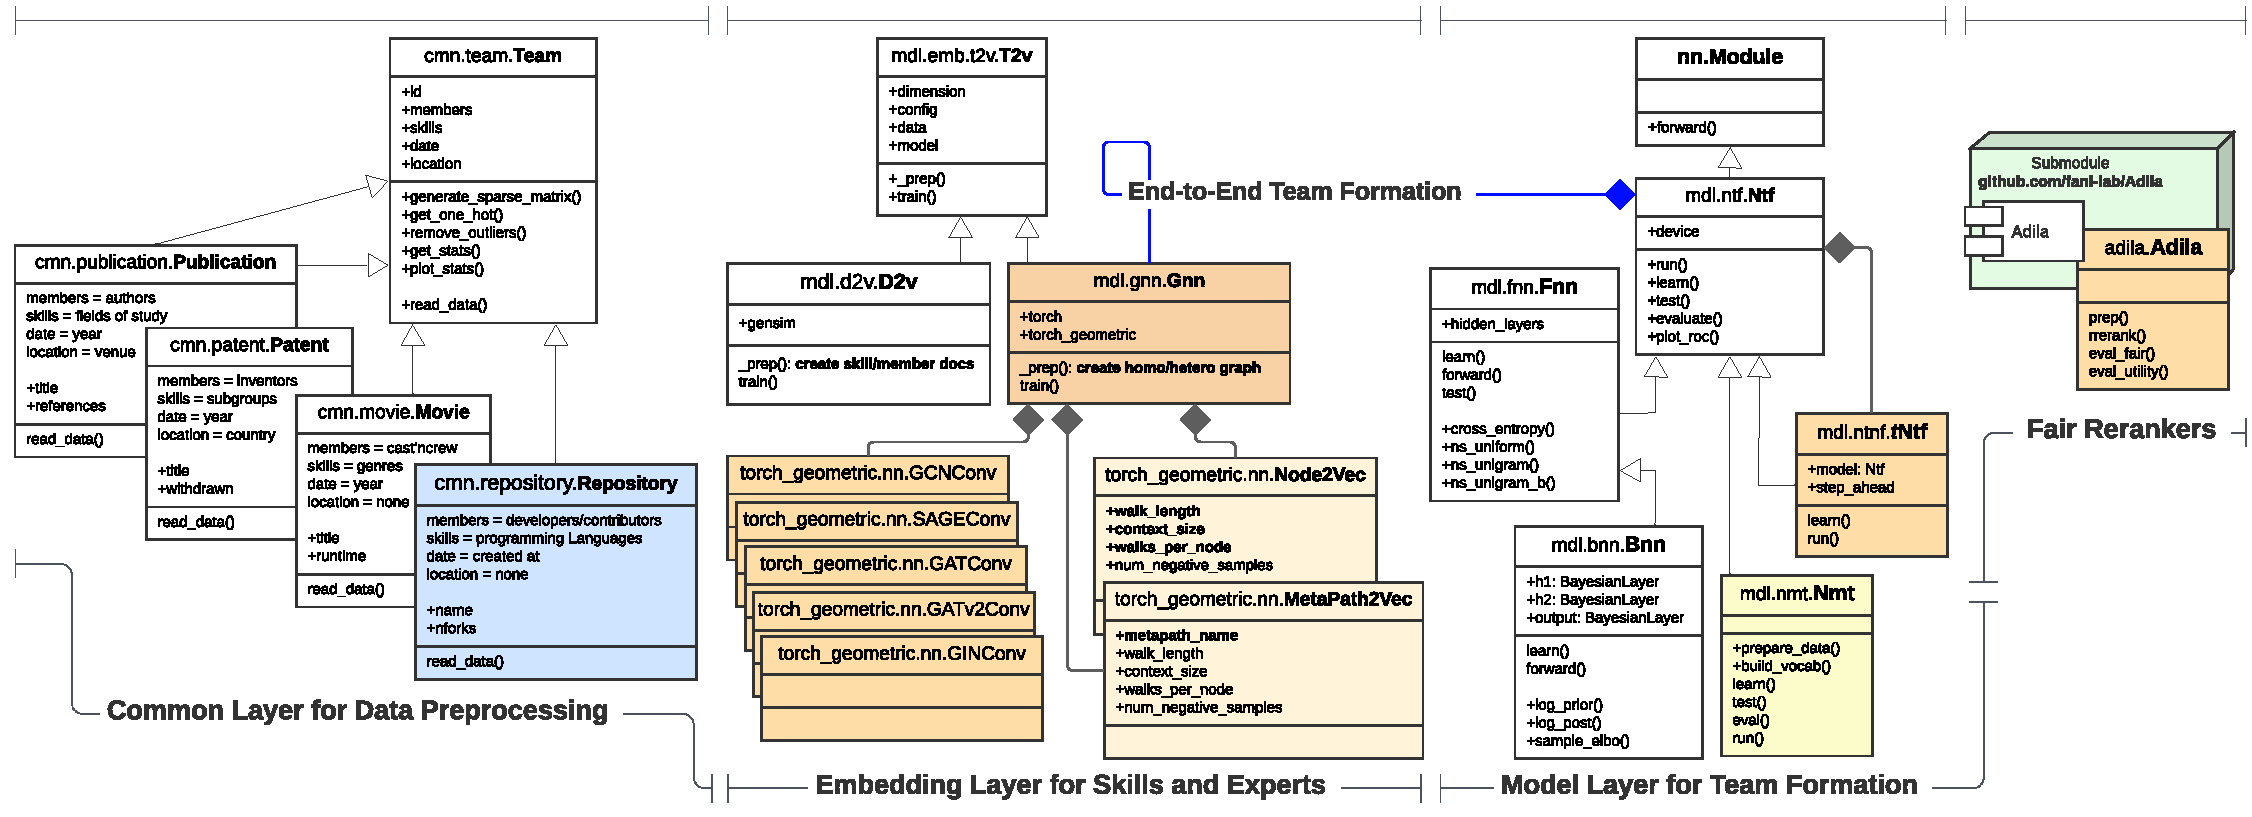
\includegraphics[width=\textwidth,height=62mm,keepaspectratio]{Images/uml.pdf}
\captionof{figure}{Architecture example supplied by the instructor (team-formation domain),
preserved as a template illustration. Replace it with your own system architecture.}
\label{architecture}
\vspace{8pt}
\end{minipage}
}]

\subsection{SELECT: Incident Timeline}
\par\noindent\begin{minipage}{\columnwidth}
\begin{lstlisting}
SELECT I.Reference, A.EventReference,
       A.OccurredAt, S.AssetCode, R.Name
FROM Incident I
JOIN Action A ON A.IncidentId = I.Id
JOIN Asset S ON S.Id = A.AssetId
LEFT JOIN Actor R ON R.Id = A.ActorId
WHERE I.Reference = 'INC-001'
ORDER BY A.OccurredAt, A.Id;
\end{lstlisting}
\end{minipage}\par
The left join retains actions with an unknown actor. With the illustrative
records above, the result associates \texttt{EVT-001} with \texttt{SRV-001}.
This is an expected example, not a measured execution result.
Evidence retrieval joins \texttt{Observation} to \texttt{Action} and then
\texttt{Incident}. A cross-incident technique query illustrates aggregation:
\par\noindent\begin{minipage}{\columnwidth}
\begin{lstlisting}
SELECT T.TechniqueCode,
       COUNT(DISTINCT A.IncidentId) AS IncidentCount
FROM Technique T
JOIN ActionTechnique X ON X.TechniqueId = T.Id
JOIN Action A ON A.Id = X.ActionId
GROUP BY T.Id, T.TechniqueCode;
\end{lstlisting}
\end{minipage}\par
DISTINCT avoids counting an incident repeatedly when several actions use the
same technique. \guidance{Prioritize SELECT queries that answer your actual
information needs; explain joins, filters, aggregation, and meaningful outputs.}

\subsection{INSERT, UPDATE, and DELETE}
\par\noindent\begin{minipage}{\columnwidth}
\begin{lstlisting}
INSERT INTO Incident
 (Reference,Title,OccurredAt,Severity,Status)
VALUES ('INC-DEMO','Synthetic example',
 '2026-10-01T10:00:00Z','Low','Open');
UPDATE Incident SET Status = 'Closed'
WHERE Reference = 'INC-DEMO';
DELETE FROM Incident WHERE Reference = 'INC-DEMO';
\end{lstlisting}
\end{minipage}\par
These statements illustrate a temporary incident without dependent records.
In an application, bind user inputs as parameters and commit successful
transactions or roll back failures. Reject missing values, invalid timestamps,
and unsupported categories. Explain how dependent records affect deletion.

\section{Architecture and User Interface}
The incident application separates forms and search controls, validation and transaction logic, and parameterized SQLite access. Results and errors return to the interface. Users can enter, search, update, and delete incidents without writing SQL; updates preserve record identity.



\guidance{Explain actual layers and information flow (Figure~\ref{architecture}); replace the UI placeholder (Figure~\ref{ui}) with screenshots of operations and results.}

\section{Reproducibility and Evaluation}
Provide separate DDL, seed data, queries, application code, and a quickstart. Document dependencies, foreign-key configuration, license, and reproduction steps. Test duplicate keys, invalid references, optional attribution, and restricted deletion; report observed results.
\guidance{Link the evaluator-accessible repository and document individual contributions and critical evaluation of AI assistance. This sample used ChatGPT~\cite{chatgpt}; students must report their own evaluation.}

\begin{thebibliography}{1}
\bibitem{chatgpt} OpenAI. 2026. ChatGPT. AI assistance for sample text,
relational design, and SQL drafting, 20 October 2026.
\end{thebibliography}

% The manual requires exactly two report pages, then one relations page.
% Compile with acmart and adjust content/figure placement; clearpage alone
% cannot guarantee the required total length.
\clearpage
\onecolumn
\section*{Relations and Constraints: Illustrative ER-to-Relational Mapping}
\small
\guidance{Replace this list with \emph{all} relations in your project. For each,
identify its autogenerated surrogate key, business candidate keys, foreign
keys, mandatory/optional attributes, and relevant domain constraints.}

An underlined \(\text{Id}\) denotes the autogenerated INTEGER primary key. CK below
lists additional business candidate keys, each enforced by UNIQUE and NOT
NULL; \(\{\text{Id}\}\) is also a candidate key in every relation. All non-key
attributes are mandatory unless explicitly marked optional. All foreign keys
reference the indicated relation's \(\text{Id}\), with no cascading deletion.
\begin{enumerate}
\item \(\text{Incident}\mathopen{(}\underline{\text{Id}},\text{Reference},\text{Title},\text{OccurredAt},\text{Severity},\text{Status}\mathclose{)}\).\\
CK: \(\{\text{Reference}\}\), mandatory. Severity \(\in\) \{Low, Medium, High, Critical\};
Status \(\in\) \{Open, Investigating, Closed\}.
\item \(\text{Actor}\mathopen{(}\underline{\text{Id}},\text{ActorCode},\text{Name},\text{Category}\mathclose{)}\).\\
CK: \(\{\text{ActorCode}\}\), mandatory. Category is mandatory text. Name need not be unique.
\item \(\text{Asset}\mathopen{(}\underline{\text{Id}},\text{AssetCode},\text{Name},\text{Kind}\mathclose{)}\).\\
CK: \(\{\text{AssetCode}\}\), mandatory. Kind is mandatory text.
\item \(\text{Technique}\mathopen{(}\underline{\text{Id}},\text{TechniqueCode},\text{Name}\mathclose{)}\).\\
CK: \(\{\text{TechniqueCode}\}\), mandatory. Codes are unique within the chosen vocabulary.
\item \(\text{Action}\mathopen{(}\underline{\text{Id}},\text{EventReference},\text{IncidentId},\text{ActorId},\text{AssetId},\text{OccurredAt},\text{Description}\mathclose{)}\).\\
CK: \(\{\text{EventReference}\}\), mandatory.\\
FK\(_1\): \(\text{IncidentId}\to \text{Incident}.\text{Id}\), mandatory;
FK\(_2\): \(\text{ActorId}\to \text{Actor}.\text{Id}\), optional;
FK\(_3\): \(\text{AssetId}\to \text{Asset}.\text{Id}\), mandatory.\\
Each action belongs to exactly one incident and targets exactly one asset.
Multiple target assets require separate target-specific actions in this sample.
\item \(\text{ActionTechnique}\mathopen{(}\underline{\text{Id}},\text{ActionId},\text{TechniqueId}\mathclose{)}\).\\
CK: \(\{\text{ActionId},\text{TechniqueId}\}\), mandatory.\\
FK\(_1\): \(\text{ActionId}\to \text{Action}.\text{Id}\), mandatory;
FK\(_2\): \(\text{TechniqueId}\to \text{Technique}.\text{Id}\), mandatory.\\
This associative relation implements the many-to-many action--technique relationship.
\item \(\text{Observation}\mathopen{(}\underline{\text{Id}},\text{EvidenceReference},\text{ActionId},\text{ObservedAt},\text{Source},\text{Detail}\mathclose{)}\).\\
CK: \(\{\text{EvidenceReference}\}\), mandatory.
FK: \(\text{ActionId}\to \text{Action}.\text{Id}\), mandatory.\\
Each observation supports exactly one action; an action may have zero or more observations.
\item \(\text{Impact}\mathopen{(}\underline{\text{Id}},\text{IncidentId},\text{AssetId},\text{Dimension},\text{Description}\mathclose{)}\).\\
CK: \(\{\text{IncidentId},\text{AssetId},\text{Dimension}\}\), mandatory.\\
FK\(_1\): \(\text{IncidentId}\to \text{Incident}.\text{Id}\), mandatory;
FK\(_2\): \(\text{AssetId}\to \text{Asset}.\text{Id}\), mandatory.\\
Dimension \(\in\) \{Confidentiality, Integrity, Availability\}. At most one summary
is stored for each incident--asset--dimension combination.
\end{enumerate}
\paragraph{Mapping assumptions.}
Incidents, actors, assets, and techniques may exist before their related rows are entered; hence parent-side participation is optional. Every action must reference an existing incident and asset. Attribution may be unknown. An impact may be recorded before the responsible action is known. Occurrence and observation times are UTC text in a fixed ISO-style format; input validation must enforce the format. Ordering timestamps does not establish causality.
\paragraph{Implementation checks.}
Use INTEGER PRIMARY KEY AUTOINCREMENT for each \(\text{Id}\) and INTEGER for foreign keys. Enable foreign-key enforcement on every connection. NOT NULL does not reject empty strings; validate these separately where empty values are not meaningful. Your DDL and report must agree about key uniqueness, NULL values, cardinalities, and delete behavior.
\end{document}
